%\iffalse
\let\negmedspace\undefined
\let\negthickspace\undefined
\documentclass[journal,12pt,onecolumn]{IEEEtran}
\usepackage{cite}
\usepackage{amsmath,amssymb,amsfonts,amsthm}
\usepackage{algorithmic}
\usepackage{graphicx}
\usepackage{textcomp}
\usepackage{xcolor}
\usepackage{txfonts}
\usepackage{listings}
\usepackage{enumitem}
\usepackage{circuitikz}
\usepackage{mathtools}
\usepackage{gensymb}
\usepackage{comment}
\usepackage[breaklinks=true]{hyperref}
\usepackage{tkz-euclide} 
\usepackage{listings}
\usepackage{gvv}    
\usepackage{enumitem}
\usepackage{amsmath}
\def\inputGnumericTable{}                                 
\usepackage[latin1]{inputenc}                                
\usepackage{color}                                            
\usepackage{array}                                            
\usepackage{longtable}                                       
\usepackage{calc}                                             
\usepackage{multirow}                                         
\usepackage{hhline}                                           
\usepackage{ifthen}                                           
\usepackage{lscape}
\usepackage{tabularx}
\usepackage[italicdiff]{physics}
\usepackage{mathrsfs}


\newtheorem{theorem}{Theorem}[section]
\newtheorem{problem}{Problem}
\newtheorem{proposition}{Proposition}[section]
\newtheorem{lemma}{Lemma}[section]
\newtheorem{corollary}[theorem]{Corollary}
\newtheorem{example}{Example}[section]
\newtheorem{definition}[problem]{Definition}
\newcommand{\BEQA}{\begin{eqnarray}}
\newcommand{\EEQA}{\end{eqnarray}}
\newcommand{\define}{\stackrel{\triangle}{=}}
\theoremstyle{remark}
\newtheorem{rem}{Remark}
\begin{document}
\bibliographystyle{IEEEtran}
\vspace{3cm}

\title{GATE:2022 - CE 48 }
\author{EE23BTECH11025 - Anantha Krishnan $^{}$% <-this % stops a space
}
\maketitle
\bigskip



\section{question}

Consider the differential equation
\begin{align}
    \frac{dy}{dx} = 4(x+2) - y \notag
\end{align}
For the initial condition $y = 3$ at $x = 1$, the value of $y$ at $x = 1.4$ obtained using Euler's method with a step-size of 0.2 is ? (\textit{round off to one decimal place})
\hfill{(GATE CE 2022)}\\
 



\textbf{Solutions :}
%\fi
\begin{table}[ht!]
\centering
\begin{tabular}{ |c|c|c| } 
 \hline
Symbols & Description & Values  \\
\hline
$R$ & Residue Formula &$\frac{1}{\brak {m-1}!}\lim\limits_{s\to a}\frac{d^{m-1}}{ds^{m-1}}\brak {{(s-a)}^{m}f\brak se^{st}}$\\
 \hline
 $\phi(x)$ & Transformation of $y(x)$ & $y(x+1)$\\
 \hline
$g(x)$ & Euler's Approximated function of f(x) & $g_{(n-1)}(x) + hf'\brak{x_{n-1},y_{n-1}}$\\
 \hline
 $h$ & Step-size & $0.2$\\
 \hline
\end{tabular}
\caption{Parameters, Descriptions, and Values}
\label{table:ee25-ce48-gate2022}
\end{table}





\begin{enumerate}
    \item Solution of the differential:\\
 Applying the transformation from table \ref{table:ee25-ce48-gate2022} and laplace transform 
    \begin{align}
             s\mathscr{L}\brak{\phi(x)} - \phi(0) &= 4\brak{\frac{1}{s^2}+\frac{3}{s}}-\mathscr{L}\brak{\phi(x)}\\
             \mathscr{L}\brak{\phi(x)} &= \frac{3}{s+1} + 4\brak{\frac{1}{s^2\brak{s+1}}+\frac{3}{s\brak{s+1}}}\\
             &=\frac{-5}{s+1} + \frac{8}{s} + \frac{4}{s^2}
    \end{align}
\item  Inverse Laplace Transform:\\
Using Bromwich integrals and extension of Jordans lemma :
\begin{align}
    \phi(t) &= \frac{1}{2\pi j}\int_{c-j\infty}^{c+j\infty}\mathscr{L}\brak{\phi(x)}e^{st}\,dt , c > 0\\
     &= \frac{1}{2\pi j}\int_{c-j\infty}^{c+j\infty}\brak{\frac{-5}{s+1} + \frac{8}{s} + \frac{4}{s^2}}e^{st}\,dt
\end{align}
Here, the poles $s=-1$ (non repeated, $m=1$) and $s=0$ (repeated, $m=2$) lie inside a semicircle for some $c>0$. Using method of residues from \ref{table:ee25-ce48-gate2022}:
\begin{align}
    R_1 &= \lim\limits_{s\to -1}\brak {{\brak{s+1}}\brak{\frac{-5}{s+1}}e^{st}} \\
    &= -5e^{-t}\\
   R_2 &= \lim\limits_{s\to 0}\brak {{\brak{s}}\brak{\frac{8}{s}}e^{st}}\\
   &= 8\\
 R_3&=\frac{1}{\brak {1}!}\lim\limits_{s\to 0}\frac{d}{dz}\brak {{(s)}^{2}\brak{\frac{4}{s^2}}e^{st}}\\
 &=4t\\
\phi(t) &= R_1 + R_2 + R_3\\
&= -5e^{-t} + 8 + 4t
\end{align}
Reverting to $y(x)$ , we get :
\begin{align}
    y(x) &= -5e^{-x+1} + 4 + 4x
\end{align}
\end{enumerate}
Now, approaching to $y(1.4)$ using euler's approximation from \ref{table:ee25-ce48-gate2022}
\begin{align}
    g_{\brak{1.2}} &= 3 + \brak{0.2}f'\brak{1,3}\\
    &=4.8\\
    g_{\brak{1.4}} &= 4.8 +\brak{0.2}f'\brak{1.2,4.8}\\
    &= 6.4\\
    &\implies y(1.4) \approx 6.4 
\end{align}





    \begin{figure}[!ht]    
    \centering
\graphicspath{ {figs/} }
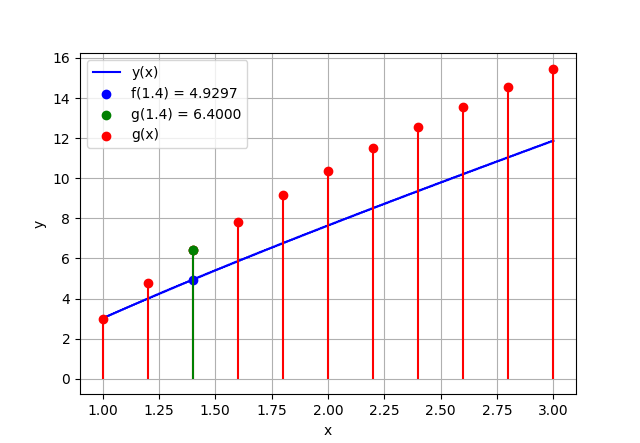
\includegraphics[width=\columnwidth]{graph_1}
\caption{ Euler's approximated function vs Original function  }
\label{graph:ee25-gate3-graph}
\end{figure}
\end{document}


